\documentclass{article}
%encoding
%--------------------------------------
\usepackage[utf8]{inputenc}
\usepackage[T1]{fontenc}
%--------------------------------------
 
%German-specific commands
%--------------------------------------
\usepackage[ngerman]{babel}
\usepackage{csquotes}
%--------------------------------------

%Pictures
%--------------------------------------
\usepackage{graphicx}
\graphicspath{ {./Pictures/} }
\usepackage{tikz}
\usepackage{subcaption}
\usepackage{float}
\usepackage{wrapfig}
%--------------------------------------

%math
%--------------------------------------
\usepackage{amsmath}
\usepackage{amssymb}
\usepackage{amsfonts}
%--------------------------------------

%Frames
%--------------------------------------
\usepackage{framed}

%Colors
%--------------------------------------
\usepackage{xcolor}
\definecolor{blue-violet}{rgb}{0.54, 0.17, 0.89}
\definecolor{codegreen}{rgb}{0,0.6,0}
\definecolor{codegray}{rgb}{0.5,0.5,0.5}
\definecolor{codepurple}{rgb}{0.58,0,0.82}
\definecolor{backcolour}{rgb}{0.95,0.95,0.92}

%--------------------------------------
\usepackage{multicol}
\usepackage[shortlabels]{enumitem}

%Aufgaben
%--------------------------------------
\usepackage{amsthm}
\newtheorem{aufgabe}{Aufgabe}[section]
\newtheorem{definition}{Definition}[section]
\newtheorem{beispiel}{Beispiel}[section]
\newtheorem*{lernaufgabe*}{Lernaufgabe}
%--------------------------------------

%Listings
%--------------------------------------
\usepackage{ulem}
\usepackage{listings}
 
\lstdefinestyle{mystyle}{
    backgroundcolor=\color{backcolour},   
    commentstyle=\color{codegreen},
    keywordstyle=\color{magenta},
    numberstyle=\tiny\color{codegray},
    stringstyle=\color{codepurple},
    basicstyle=\ttfamily\footnotesize,
    breakatwhitespace=false,         
    breaklines=true,                 
    captionpos=b,                    
    keepspaces=true,                 
    numbers=left,                    
    numbersep=5pt,                  
    showspaces=false,                
    showstringspaces=false,
    showtabs=false,                  
    tabsize=2,
}
 
\lstset{style=mystyle,moredelim=[is][\sout]{|}{|}}
%--------------------------------------


\title{Fliesskommazahlen -- Unterrichtskonzeption}
\author{Alexandra Maximova}
\date{FS2020}

\begin{document}

\maketitle


\section*{Rahmenbedingungen}
Die LPU richtet sich an SuS, die das zweite Semester des Ergänzungsfachs Informatik absolvieren. Die SuS haben Physik und angewandte Mathematik als Schwepunktfach gewählt, und haben keine besondere Mühe mit Mathematik.

Die Fliesskommazahlen sind das zweite Thema im Modul \textbf{'Daten Darstellen'}. In diesem Modul beschäftigen wir uns grundsätzlich mit der Frage, warum man sagt, dass im Computer nur Nullen und Einser gespeichert werden, wenn wir doch alle sehen, dass im Computer Texte, Bilder und Videos gespeichert werden, die auf dem ersten Blick gar nichts mit Nullen und Einser zu tun haben. Das erste Thema des Moduls 'Daten Darstellen' waren ganze Zahlen. Die SuS haben die Zweierkomplement-Darstellung kennengelernt.

Diese LPU umfasst die zweite und dritte Stunde zum Thema Fliesskommazahlen. In der ersten Stunde, die nur kurz aufgefrischt wird, wurden die Fliesskommazahlen eingeführt und die Metapher  vom Kasten und Seil präsentiert. Diese Metapher ist unten genauer beschrieben.

\section*{Stoffanalyse}
\begin{figure}[H]
\centering
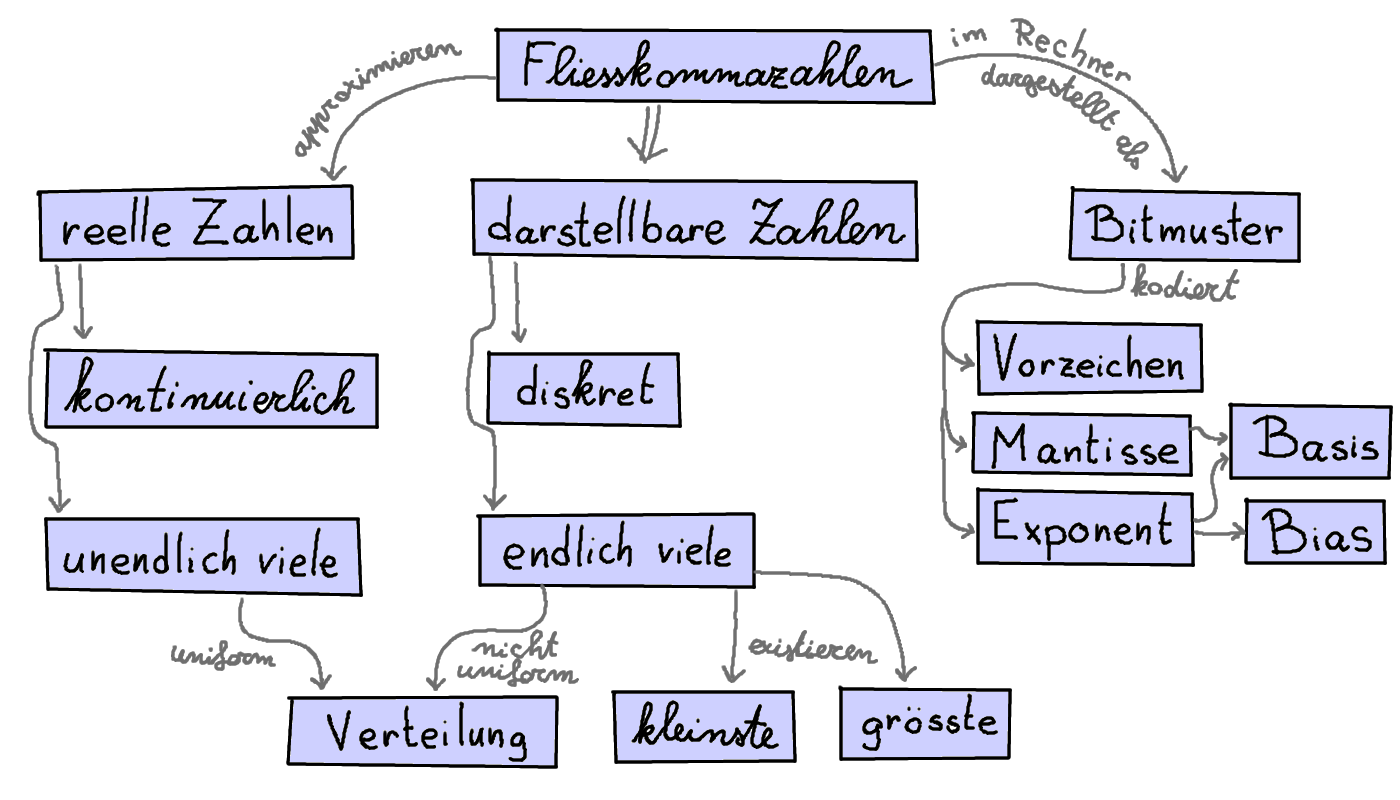
\includegraphics[width=\textwidth]{Pictures/Fliesskommazahlen_Concept_Map.png} 
\end{figure}

Die \textbf{Fliesskommazahlen} werden eingesetzt, um \textbf{reelle Zahlen} zu approximieren. Die reelle Zahlen werden in der Exponentialdarstellung in Basis 2 als \(x = (-1)^s m \cdot 2^e\) geschrieben, wobei \(s\) das \textbf{Vorzeichen} kodiert,

Fokus
Hier ist der Fokus auf die Verteilung von Fliesskommazahlen auf dem Zahlenstrahl. Wo sind sie näher zueinander, wo sind sie weiter voneinander, was ist die kleinste und die grösste Zahl, was sind die Nachbarzahlen.
Mit der Arche schauen die SuS, was für Zahlen sind das, wie viele davon es gibt, was ist die grösste und die kleinste und wo sind sie auf dem Zahlenstrahl.

\subsection*{Metapher vom Kasten und Seil}

       Die SuS haben ausserdem in der vorherigen Stunde ein mechanisches Modell von Fliesskommazahlen gesehen, bestehend aus einem Holzkasten (Mantisse) mit einem Seil (Exponent).  Dieses Modell wird in dieser Stunde verwendet, um die Fliesskommazahlen besser kennenzulernen.
       Mit dem Kasten suchen die SuS die grösste und kleinste darstellbare Zahl, den Abstand zwischen benachbarten darstellbaren Zahlen und lernen, Fliesskommazahlen zu addieren. Bei der Addition sehen sie auch zwei Beispiele, wo das Ergebnis im Fliesskommazahlensystem mit der Intuition, die man aus den reellen Zahlen hat, nicht übereinstimmt.
Didaktische Varianten:
- Eiskapseln wie in Raumschiffe, um Zahlen einzufrieren, so dass sie weniger Platz bei der Transportierung brauchen. Damit sie wieder aufgetaut werden können, muss man wissen, wo man sie bezüglich dem Komma anpflanzen muss.
- Die Arche Noah. Die Zahlen werden von der grossen Flut gerettet. Für jede Zahl, die wir retten wollen, konstruieren wir so eine Arche. Aber es haben nicht alle Ziffern Platz. Welche nehmen wir ans Bord? Ziffern sind nicht alles, was wir brauchen, um die Zahl wieder zu rekonstruieren (dorthin zu bringen, wo sie war?). Wir brauchen auch das Seil mit dem Anker. Und natürlich werden solche Archen in einer Fabrik produziert, also haben wir mega viele davon, sind aber alle gleich (haben gleich viele Plätze und das Seil mit dem Anker ist gleich lang; das einzige, was wir ändern können, ist Anker umhängen). (Deswegen heissen sie ja Fliesskommazahlen).


\section*{Vorwissen}
       - sie können programmieren, aber das ist hier nicht wichtig
       - sie kennen Integers und Two’s Complement
       - sie kennen die Exponentialdarstellung (Chemie, Physik)
       - sie haben die Struktur (Vorzeichen, Mantisse, Exponent) von Fliesskommazahlen und die Metapher vom Kasten und Seil die Stunde davor gesehen
       Die LPU ist an SuS der Gymnasialstufe gerichtet. Das ist die zweite Stunde über Fliesskommazahlen. Ausserdem wissen die SuS schon, wie man Integer im Computer darstellt.
       Folgende Themen werden als Vorwissen angenommen und, wenn nötig, aufgefrischt:
       1. Exponentialdarstellung von Dezimalzahlen in Basis 10 (bekannt aus Chemie und Physik) Vorzeichen, Exponent, Mantisse, Basis
       2. Exponentialdarstellung von Dezimalzahlen in Basis 2, insbesondere ganze und rationale Zahlen in Binär umwandeln.

\section*{Lernziele}

\paragraph{Leitidee} Die SuS können nachvollziehen, wie der Computer “zaubert”.

\paragraph{Dispositionsziel} Die SuS vertrauen nicht mehr blind einem Computer bei Berechnungen mit reellen Zahlen.

\paragraph{Operationalisierte Lernziele}
\begin{itemize}
\item Die SuS finden die grösste und kleinste Zahl in einem Fliesskommazahlensystem.
\item Gegeben eine Fliesskommazahl, die SuS schreiben die nächste und die vorherige darstellbare Zahl auf.
\item Die SuS addieren zwei gegebene Fliesskommazahlen.
\end{itemize}




\end{document}
